\chapter{Design}

\section{Introduction}

The design of Tourlingo aimed to design not just a map-based website, but a multilingual and culturally sensitive travel assistant. Our design process focused on helping international travellers feel more comfortable and confident in unfamiliar environments by providing accessible, local information in their preferred language.

To achieve our goal, we followed a user-centred design approach, using wireframing and interactive prototyping to explore key features. We then conducted early user evaluation through a think-aloud method, which informed several improvements to the initial prototype. The following sections describe our design requirements, UX process and early-stage evaluation in more detail.

\section{Design Requirements}

\subsection{Overview}
To ensure that our product effectively supports international tourists navigating unfamiliar environments, we began the design by analysing client's requirements and aligning them with User-Centred Design (UCD) principles. The client's initial product vision highlighted the importance of multilingual support, local cultural guidance and user-friendly User Interface (UI). Based on these inputs, we carried out a systematic prioritisation process to define our Product Requirements Document (PRD) and Minimum Viable Product (MVP).

\subsection{Client Side Requirements}
The project began with a clear set of high-level requirements proposed by the client \textbf{\textcolor{red}{(can refer to the screenshot of the email from the client)}}, aiming to assist international tourists in navigating unfamiliar environments. These requirements served as the foundation of our design process and were categorised into six key areas:

\begin{itemize}
    \item \textbf{Web-Based and Cross-Device Compatibility}: Instead of developing a native app that requires downloading, the product should be built as a mobile-responsive website. This allows users to access the application instantly without registration or installation. The product should support both smartphone and desktop devices, allowing users to access the website flexibly based on their device of choice.
    \item \textbf{Language Selection and Multilingual Support}: Users should be able to select their preferred language at the beginning of their session, and the application should then present the contents in the selected language.
    \item \textbf{Location-Based Service Recommendations}: GPS functionality should be used to identify and display nearby essential services such as public transport hubs, hospitals, ATMs, and stores. The product optionally provides real-time navigation and estimated arrival times to these services.
    \item \textbf{Local Information and Cultural Tips}: The application should display culturally relevant tips, such as local etiquette, useful phrases, and customs, to help travellers adapt and avoid misunderstandings. Local emergency services and tourist hotlines should be available as well.
    \item \textbf{User-Friendly and Accessible Design}: The interface should be simplified for ease of use by individuals of various ages and digital literacy levels. Where feasible, accessibility features such as text-to-speech should be included to assist users with visual impairments.
    \item \textbf{Optional Natural Language Features}: If time permits, natural language processing (NLP) features could be integrated.
\end{itemize}


\subsection{User-Centred Design Requirements}
To ensure our design process was guided by real user needs, we adopted the User-Centred Design (UCD) approach. UCD is defined as an iterative process that places users at the core of each development stage, aiming to improve usability and satisfaction by focusing on how users interact with the product \cite{ux_ucd_interaction}. It has been widely used in digital applications due to its ability to reduce cognitive load, enhance accessibility and deliver solutions aligned with users' expectations.

Given the international and multicultural nature of our product, UCD was especially appropriate. It allowed us to design not only for functionality, but also for empathy-addressing needs such as multilingual users, cultural awareness, and ease of use across different cultural backgrounds. Importantly, our team itself consists of international students from diverse cultural backgrounds, which enabled us to bring multiple user perspectives into the design process and more intuitively consider the needs of global travellers.

According to the UCD principles, there are four stages: understanding the users and context, specifying user needs, producing design solutions, and evaluating those solutions through testing. As we were unable to directly involve real users during the early phase of the project, we positioned ourselves as representative users by analysing the client's requirements from a user perspective. Each team member translated the functional expectations into short, clear user stories \textbf{\textcolor{red}{(add reference to the appendix of the user story file)}}. These user stories helped us empathise with end users and served as the foundation for creating the potential features and UI elements. We then merged individual user stories into a combined file and used them to explore design directions.

\subsection{Requirements Documentation and MVP} 
Following the user stories and internal brainstorming, we compiled a formal Product Requirements Document (PRD), which outlined both functional and non-functional design for our proposed solution (see Appendix~\ref{appendix:prd}). During subsequent meetings with the client and our supervisor, we discussed the feasibility of each proposed feature. Ultimately, we agreed on delivering a Minimum Viable Product (MVP) that would form the foundation for future extensions. 

The MVP included the following five core components: 
\begin{itemize} 
    \item \textbf{Language Selection Page}: Allows users to choose their preferred language for accessing the application, and can change language at anytime. 
    \item \textbf{Map Page}: Enables users to search locations, receive basic navigation support, and show pins of the section items in map. 
    \item \textbf{Recommendation Page}: Shows restaurants, stores and so on near the current or searched location. 
    \item \textbf{Essential Page}: Offers location-based information like pharmacies, hospitals, police stations and so on. 
    \item \textbf{Cultural Tips Page}: Provides culturally sensitive content such as etiquette, local phrases, transportation and payment methods and other practical information. 
\end{itemize} 

The overall structure of these components is illustrated in Figure~\ref{fig:frontend-flowchart}.

\begin{figure}[H] 
    \centering 
    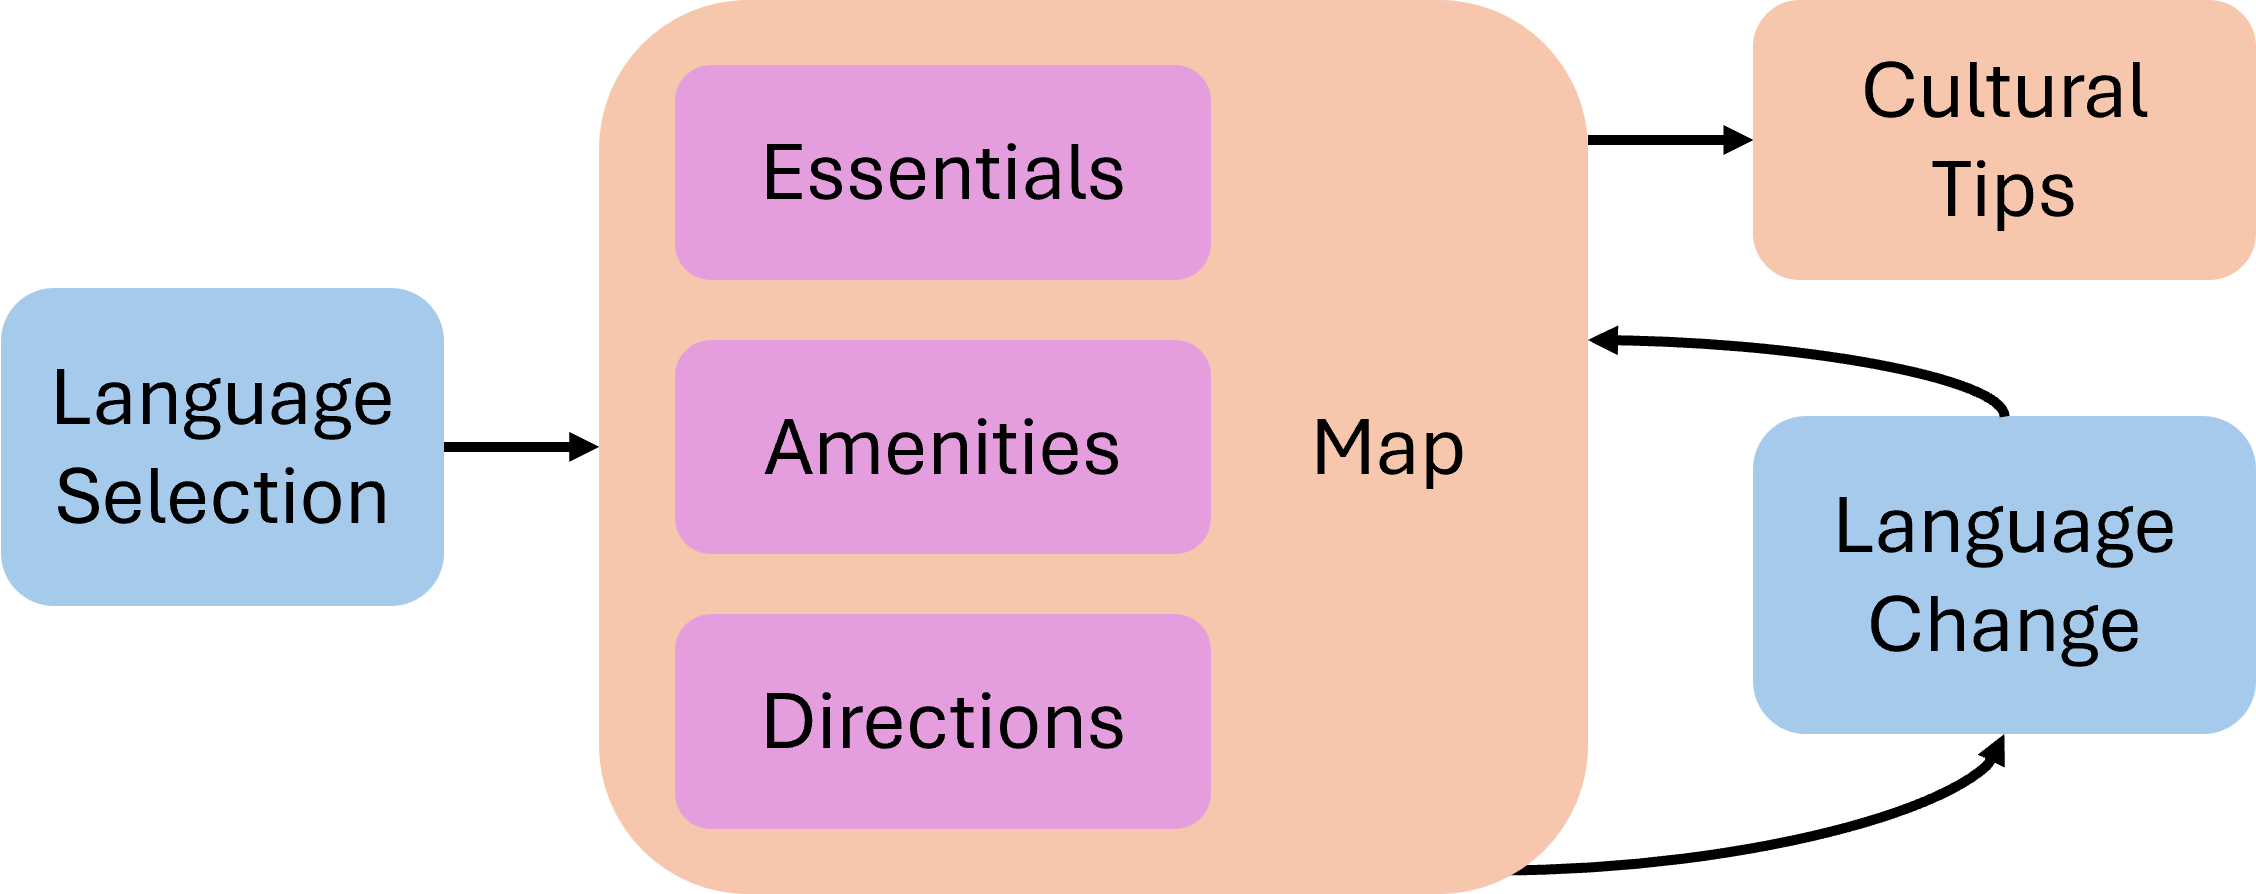
\includegraphics[width=0.5\textwidth]{images/Frontend/Frontend_Flowchart.png} 
    \caption{Frontend flowchart} 
    \label{fig:frontend-flowchart} 
\end{figure} 

The product was designed as a responsive web application, rather than a mobile app. This ensures users can simply open a link or enter the URL without needing to download or register. It also facilitates usage in transportation stations like airports or train stations, aligning well with the 'use and go' nature of our product.

\section{Wireframing and User Experience (UX)}

\subsection{Purpose of Using Wireframing}
Wireframing served as a foundational step in our design process, allowing us to explore layout, interaction flow, and feature prioritisation before committing to development. The purpose was to visualise the user journey, test early hypotheses about interface design, and facilitate communication within the team.

We used Figma as our primary tool for wireframing due to its collaborative features and ease of use.

\subsection{Inspiration and Design Exploration}
To begin our UI design process, the team explored several design websites for inspiration, including Dribbble, Mobbin \textbf{\textcolor{red}{(add reference of the website link)}}. These resources provided a wide range of mobile and web UI/UX patterns, enabling us to understand current trends in travel and map-based applications.

\subsection{Initial Wireframing and UX Consideration}
Based on the inspirations collected, one of our team members took the lead on the UI design by producing initial wireframes. These wireframes were created using Figma and focused on the overall structure and layout of the key pages in both mobile and desktop views. The wireframes defined the content hierarchy, navigation structure, and component placement before any styling decisions were made.

Throughout the wireframing stages, several UX principles guided our design choices:
    \begin{itemize}
        \item \textbf{Clarity and Simplicity}: Ensuring the UI is approachable for users of different age groups and technological backgrounds.
        \item \textbf{Accessibility}: Maintaining sufficient colour contrast, clear labelling, and considering potential for future features like text-to-speech.
        \item \textbf{Consistency}: Preserving consistent layout and behaviour across screens to reduce cognitive load.
    \end{itemize}

\textbf{\textcolor{red}{insert pics of the wireframing for both mobile and desktop views}}


\section{Prototyping and Early Evaluation}
Building on the wireframes, we created an interactive high-fidelity prototype using Figma. Our approach aimed to visualise the complete flow of the application, enabling realistic testing of the UI and interactions.

Our prototype focused on five core screens defined in the MVP: (1) language selection, (2) interactive map, (3) recommendation page, (4) essentials page, and (5) cultural tips page. These reflected the client's priorities and user-centred insights gathered during requirement analysis.

We conducted an early evaluation using the Think-Aloud \textbf{\textcolor{red}{(should we find a reference article for think-aloud method?)}} method with a small group of student peers. Participants were asked to perform specific tasks (e.g., finding the nearest pharmacy or locating cultural etiquette tips) while verbalising their thought process. This allowed us to gather immediate feedback on usability issues and know where to improve. We wrote a feedback report after the Think-Aloud evaluation \textbf{\textcolor{red}{(add reference to the initial evaluation report appendix)}}.

\textbf{\textcolor{red}{(add pics of the prototypes)}}

Based on these evaluations, we made several changes, such as modifying the misunderstood words, changing the cultural tips page interface, and adding distance from the current location to the searched location in the navigation panel.

\textbf{\textcolor{red}{(add pics of the prototypes after early evaluation)}}

